\begin{frame}{Key Findings}
    \framesubtitle{Takeaways across both environments}
    % --- Slide 1: only left column ---
    \begin{columns}[T,onlytextwidth]
        \begin{column}{0.5\textwidth}
            \textbf{\faCheckCircle~~What works}
            \begin{itemize}
                \item \scriptsize Even smaller models can autonomously run \textbf{standard red-team reconnaissance}
                \item \scriptsize \textbf{Multi-agent decomposition} helps smaller models (--68\% tokens for \texttt{qwen3:30b})
                \item \scriptsize AI delivers \textbf{depth}: assessment, prioritized findings, remediation
            \end{itemize}
        \end{column}
        \begin{column}{0.5\textwidth}
        \end{column}
    \end{columns}
    \vspace{0.5em}
    % --- Slide 2: right column appears ---
    \begin{onlyenv}<2->
        \begin{columns}[T,onlytextwidth]
            \begin{column}{0.5\textwidth}
            \end{column}
            \begin{column}{0.5\textwidth}
                \textbf{\faExclamationTriangle~~What limits it}
                \begin{itemize}
                    \item \scriptsize \textbf{High failure rate} -- best-case subset
                    \item \scriptsize \textbf{Hallucinations}: fabricated CVEs, honeypots
                \end{itemize}
            \end{column}
        \end{columns}
    \end{onlyenv}
\end{frame}

\begin{frame}{Answering the Research Questions}
    \footnotesize
    \begin{itemize}[<+->]
        \item[\textbf{RQ1}] \textbf{AI vs.\ static:} Same discovery power as baseline, no gains in speed/determinism.
        Adds value via \textbf{reasoning and interpretation} (credentials, banner reasoning, severity scoring).
        \vspace{0.2em}
        \item[\textbf{RQ2}] \textbf{Operator support:} Converts scans into structured, severity-ranked output + next steps.
        \texttt{--interactive} Operator stays in the loop and control.
        \vspace{0.2em}
        \item[\textbf{RQ3}] \textbf{Deployment:} Scales to $\sim$35 hosts, highlights key risks.
        \textbf{Requires supervision} (reliability limits).
    \end{itemize}
\end{frame}

\begin{frame}{Project Goals}
    \framesubtitle{Order of implementation: Must $\rightarrow$ Should $\rightarrow$ Could}

    \centering
    \begin{tikzpicture}[font=\scriptsize,
        dot/.style={circle,fill,inner sep=2.2pt},
        phase/.style={font=\footnotesize\bfseries},
        goals/.style={anchor=north,align=left,text width=3.7cm}]

        % --- timeline axis ---
        \draw[->,line width=1.4pt,gray!70] (-5.6,0) -- (5.8,0);

        % ===== MUST (all achieved) =====
        \begin{scope}
            \draw[red!75!black] (-4,0) -- (-4,-0.55);
            \node[dot,red!75!black] at (-4,0) {};
            \node[phase,red!75!black,above=2pt] at (-4,0.05) {Must};
            \node[goals] at (-3.5,-0.6) {
                Compare Frameworks~\uncover<2->{{\color{green!60!black}\faCheck}}\\
                AI Integration Research~\uncover<2->{{\color{green!60!black}\faCheck}}\\
                Configuration Management~\uncover<2->{{\color{green!60!black}\faCheck}}\\
                AI Scenarios~\uncover<2->{{\color{green!60!black}\faCheck}}\\
                Reproducible Test Env.~\uncover<2->{{\color{green!60!black}\faCheck}}\\
                Red Team Reconnaissance~\uncover<2->{{\color{green!60!black}\faCheck}}\\
                AI Scenario Evaluation~\uncover<2->{{\color{green!60!black}\faCheck}}\\
                AI vs.\ Engineered (Red)~\uncover<2->{{\color{green!60!black}\faCheck}}};
        \end{scope}

        % ===== SHOULD =====
        \begin{scope}
            \draw[orange] (0.2,0) -- (0.2,-0.55);
            \node[dot,orange] at (0.2,0) {};
            \node[phase,orange,above=2pt] at (0.2,0.05) {Should};
            \node[goals] at (0.6,-0.6) {
                Blue Team Intrusion Detection\\
                AI vs.\ Engineered (Blue)};
        \end{scope}

        % ===== COULD =====
        \begin{scope}
            \draw[gray!60] (4.2,0) -- (4.2,-0.55);
            \node[dot,gray!60] at (4.2,0) {};
            \node[phase,gray!60!black,above=2pt] at (4.2,0.05) {Could};
            \node[goals] at (5.2,-0.6) {
                REST API\\
                MCP Server\\
                Web GUI};
        \end{scope}
    \end{tikzpicture}
\end{frame}

\begin{frame}{Recommendations and Future Work}
    \framesubtitle{}
    \begin{columns}[T,onlytextwidth]
        \begin{column}{0.5\textwidth}
            \textbf{Recommendations}
            \begin{itemize}
                \item \scriptsize \textbf{Match model tier to task} -- frontier model for autonomous recon
                \item \scriptsize \textbf{Multi-agent} for smaller / self-hosted models
                \item \scriptsize \textbf{Hybrid pipeline}: static breadth + AI depth (+ RAG)
                \item \scriptsize \textbf{Human-in-the-loop} + retry on incomplete runs
            \end{itemize}
        \end{column}
        \begin{column}{0.5\textwidth}
            \textbf{Future work}
            \begin{itemize}
                \item \scriptsize \textbf{Dynamic tool calling} -- expose only relevant tools
                \item \scriptsize \textbf{Guardrails \& sandboxing} -- scope restriction for production
                \item \scriptsize Robust \textbf{HITL middleware}
                \item \scriptsize \textbf{Broader attack-chain} coverage beyond reconnaissance
            \end{itemize}
        \end{column}
    \end{columns}
\end{frame}

\begin{frame}{Conclusion}
    \framesubtitle{Agentic AI complements deterministic enumeration}
    \begin{itemize}
        \item[\faCheck] Using NSAK directly as an \textbf{agentic harness} proved effective -- the agent autonomously and interactively executes network discovery via LangChain tools.
        \item[\faCheck] Scripted scenarios excel in correctness and completeness; the agent adds \textbf{reasoning and assessment}, limited by model capability.
        \item[\faCheck] \textbf{Multi-agent decomposition} models to digest large context improves models by reducing context complexity and increasing consistency.
        \item[\faExclamationTriangle] Hallucinations remain a limitation -- \textbf{supervised operation with a human reviewer} is the proposed deployment model.
    \end{itemize}
    \vspace{0.5em}
    \begin{center}
        \footnotesize\textit{LLMs make cybersecurity use cases more accessible and cost-effective -- with a human in the loop.}
    \end{center}
\end{frame}

\begin{frame}{Personal Conclusion}
    \framesubtitle{}
    \begin{columns}[T,onlytextwidth]
        \begin{column}{0.5\textwidth}
            \textbf{Frank}
            \begin{itemize}
                \item
            \end{itemize}
        \end{column}
        \begin{column}{0.5\textwidth}
            \textbf{Lukas}
            \begin{itemize}
                \item Initially skeptical of the usefulness of AI
                \item We covered a lot of topics we learned at BFH
                \item A bit of naivety in the planning led to a larger scope
                \item Keep focusing on the goals and research questions
                \item AI is here to stay as another engineering tool
            \end{itemize}
        \end{column}
    \end{columns}
\end{frame}

\section[Demo]{Demo: Agentic Reconnaissance in Action}\label{sec:demo-and-questions}
